%!TEX program=xelatex

% 碰到Windows版本提示Fandol字体,可以在命令行中以管理员权限执行:tlmgr update -self -all
%\documentclass[review]{cvpr}
\documentclass[final]{cvpr}

\usepackage[UTF8]{ctex}

%\usepackage{cvpr}
\usepackage{times}
\usepackage{epsfig}
\usepackage{graphicx}
\usepackage{amsmath}
\usepackage{amssymb}
\usepackage{subfigure}
\usepackage{overpic}
% \usepackage{float}
\usepackage{stfloats}
\usepackage{enumitem}
\usepackage[noend]{algpseudocode}   %
\usepackage{setspace}   %
\setenumerate[1]{itemsep=0pt,partopsep=0pt,parsep=\parskip,topsep=5pt}
\setitemize[1]{itemsep=0pt,partopsep=0pt,parsep=\parskip,topsep=5pt}
\setdescription{itemsep=0pt,partopsep=0pt,parsep=\parskip,topsep=5pt}


\usepackage[pagebackref=true,breaklinks=true,colorlinks,bookmarks=false]{hyperref}


%\cvprfinalcopy % *** Uncomment this line for the final submission

\def\cvprPaperID{159} % *** Enter the CVPR Paper ID here
\def\confYear{CVPR 2020}
\def\httilde{\mbox{\tt\raisebox{-.5ex}{\symbol{126}}}}

\newcommand{\cmm}[1]{\textcolor[rgb]{0,0.6,0}{CMM: #1}}
\newcommand{\todo}[1]{{\textcolor{red}{\bf [#1]}}}
\newcommand{\alert}[1]{\textcolor[rgb]{.6,0,0}{#1}}

\newcommand{\IT}{IT\cite{98pami/Itti}}
\newcommand{\MZ}{MZ\cite{03ACMMM/Ma_Contrast-based}}
\newcommand{\GB}{GB\cite{conf/nips/HarelKP06}}
\newcommand{\SR}{SR\cite{07cvpr/hou_SpectralResidual}}
\newcommand{\FT}{FT\cite{09cvpr/Achanta_FTSaliency}}
\newcommand{\CA}{CA\cite{10cvpr/goferman_context}}
\newcommand{\LC}{LC\cite{06acmmm/ZhaiS_spatiotemporal}}
\newcommand{\AC}{AC\cite{08cvs/achanta_salient}}
\newcommand{\HC}{HC-maps }
\newcommand{\RC}{RC-maps }
\newcommand{\Lab}{$L^*a^*b^*$}
\newcommand{\mypara}[1]{\paragraph{#1.}}

\graphicspath{{figures/}}

% Pages are numbered in submission mode, and unnumbered in camera-ready
%\ifcvprfinal\pagestyle{empty}\fi
\setcounter{page}{1}


\renewcommand{\figref}[1]{图\ref{#1}}
\renewcommand{\tabref}[1]{表\ref{#1}}
\renewcommand{\equref}[1]{式\ref{#1}}
\renewcommand{\secref}[1]{第\ref{#1}节}
\def\abstract{\centerline{\large\bf 摘要} \hspace*{12pt} \it}

%%%%%%%%% TITLE 

\title{伪装物体检测}

% \maketitle 

\author{Deng-Ping Fan$^{1,2}$\quad Ge-Peng Ji$^{3}$ \quad Guolei Sun$^{4}$
    \quad Jianbing Shen$^{1,}$\thanks{通讯作者:Jianbing Shen (shenjianbingcg@gmail.com)}  \quad Ling Shao$^{1}$  \\
    $^{1}$ Inception Institute of Artificial Intelligence, UAE \quad$^{2}$College of CS, Nankai University, China\\
    \quad$^{3}$ School of Computer Science,Wuhan University, China \quad $^4$ETH Zurich, Switzerland 
}

\maketitle    %能用的位置
\begin{document}

\begin{figure*}[tp]%这个好像成了
\centering
\subfigure
{
    \begin{minipage}[htbp]{.18\linewidth}
        \centering
        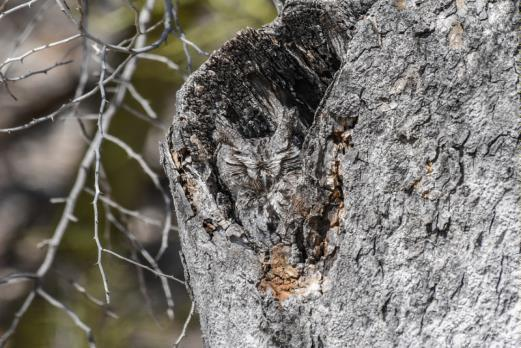
\includegraphics[scale=0.25]{COD_Zh_translate/figures/example1.png}
        \hspace{5mm} %调整纵向距离
    \end{minipage}
}
\subfigure
{
 	\begin{minipage}[htbp]{.18\linewidth}
        \centering
        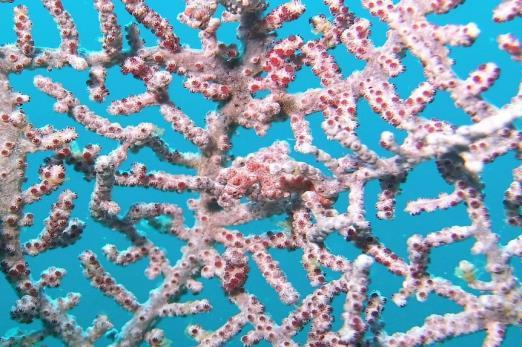
\includegraphics[scale=0.25]{COD_Zh_translate/figures/example2.png}
        \hspace{5mm} %调整纵向距离
    \end{minipage}
}
\subfigure
{
 	\begin{minipage}[htbp]{.18\linewidth}
        \centering
        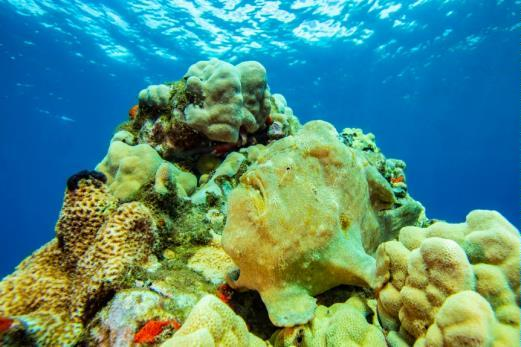
\includegraphics[scale=0.25]{COD_Zh_translate/figures/example3.png}
        \hspace{5mm} %调整纵向距离
    \end{minipage}
}
\subfigure
{
 	\begin{minipage}[htbp]{.18\linewidth}
        \centering
        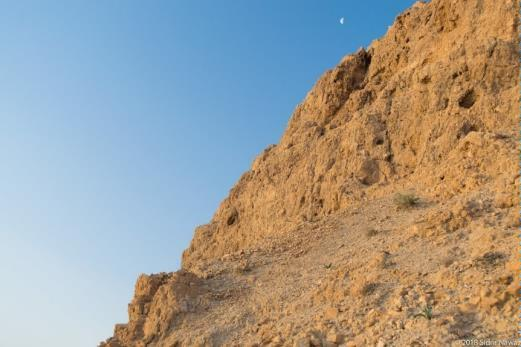
\includegraphics[scale=0.25]{COD_Zh_translate/figures/example4.png}
        \hspace{5mm} %调整纵向距离
    \end{minipage}
}
\subfigure
{
 	\begin{minipage}[htbp]{.18\linewidth}
        \centering
        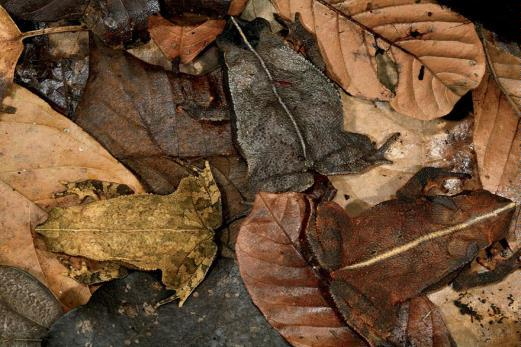
\includegraphics[scale=0.25]{COD_Zh_translate/figures/example5.png}
        \hspace{5mm} %调整纵向距离
    \end{minipage}
}
\caption{COD10K 数据集示例图。你能找到隐藏在图片中的伪装物体吗?以彩色电子版阅览时视觉效果最佳。 答案见补充材料。}
\label{fig:COD10K_examples}
\end{figure*}


%%%%%%%%% ABSTRACT%%%%%%%%%%%
\begin{abstract}
伪装物体检测(Camouflaged Object Detection, COD),顾名思义,旨在识别“无缝”嵌入其周围环境 的物体,本文对这项新任务展开了全面的研究。与传 统的物体检测相比,通常伪装物体与其背景之间具 有高度相似性,因此伪装物体检测更具挑战。为解决 这一问题,本文精心构建了 COD10K 数据集,它包 含了 10,000 张图像,且涵盖了各种自然场景,具有超过78个类别的伪装物体。所有的图像都进行了稠密的标注,包括类别、包围盒、对象级/实例级,以及抠图级的标签。COD10K 数据集可以助力许多视觉任务,例如目标定位、图像分割和抠图技术等。同时, 本文也为伪装物体检测任务提供了一个简单且有效 的框架,称为搜索识别网络(Search Identification Network,SINet)。没有借助过多技巧,SINet 在所有 数据集上的表现均优于其它先进的物体检测基准模 型。因此,SINet 是一个鲁棒的、通用的架构,这有助 于促进伪装物体检测的发展。最后,通过对 13 种最 先进模型进行系统评估,本文给出了许多有趣的发 现并且展示了一些伪装物体检测的潜在应用。希望 本文的研究能为这一新领域的学者提供更多探索机 会。详见:https://github.com/DengPingFan/SINet/
\end{abstract}



%%%%%%%%% BODY TEXT %%%%%%%%%%%%%%%%%%%%%%%%%%%%%%%%%%%%%%%%
\section{引言}\label{sec:Introduction}
你能在\figref{fig:COD10K_examples}中找到伪装的物体吗?生物学家将
\\
\\
\\
\\
\\
这类伪装方式称为背景匹配,即动物为避免被识别 [49],会尝试改变其自身颜色以“完美”地融入周围 环境。感官生态学家的研究表明,这种伪装策略是通 过欺骗观察者的视觉感知系统而产生的 [58]。因此, 解决伪装物体检测(Camouflaged Object Detection COD)任务需要大量的视觉感知知识 [61]。

\begin{figure}[h!]
  \begin{overpic}[width=\columnwidth]{Comparison_COD.png} \small
  \put(6,-4){(a)原图}
  \put(26,-4){(b)通用物体}
  \put(52,-4){(c)显著物体}
  \put(76,-4){(d)伪装物体}
    \end{overpic}\\
    \caption{给定一张输入图像(a),(b)为全景分割 [31] 的真值(全景分割检测中的通用物体 [40,45]包括stuff和things),(c)是显著实例/物体检测 [17, 34, 62, 77](检测最吸引人注意力的目标),(d)是本文提出的伪装物体检测任务,即检测出与 周围环境具有相似模式(例如边缘,纹理或颜色)的物体。如 图所示,两只蝴蝶的边缘与香蕉融合在一起,难以识别。
    }\label{fig:Comparsion_COD_SOD}
\end{figure}

如\figref{fig:Comparsion_COD_SOD}所 示,物体物与背景之间高度的相似性使 COD 远比 传统的显著物体检测(SOD)[1, 5, 18, 26, 63–67, 69] 或通用物体检测(GOD)[4,80] 更具挑战性。
除了其学术价值外,伪装物体检测还有助于推 动下列领域的实际应用:计算觉领域(可用于搜索 和救援工作,或寻找稀有物种)、医学图像分析领域
(如息肉分割 [15] 和肺炎分割 [19,68])、农业领域 (如蝗虫入侵监控)和艺术领域(用于真实感图像融
合 [22] 或艺术消遣 [6])。
目前,由于缺乏规模足够大的数据集,伪装物 体检测的研究还不够深入。为了对 COD 课题进行
全面的研究,本文做出了两项
\\
\\
\\
\\
\\
\\
\\
贡献。首先,本文专门 为 COD 任务精心构建了 COD10K 数据集。它与 现有的数据集有以下方面的区别:
• COD10K 数据集包含了 1 万张图像,涵盖了 78 种伪装物体类别,属于水生、飞行、两栖和 陆地等。
• 所有的伪装图像都赋予了不同的层级标签,如 类别、包围盒、对象级和实例级。这些标签会使 得许多视觉任务受益,如目标定位,似物性检 测,语义边缘检测 [43],任务迁移学习 [70] 等。
• 每张伪装图像都加上了真实环境中遇到的具有 挑战的属性以及抠图级 [74](标注一张图像耗时 约 60 分钟)的标签。这些高质量的标注有助于 对算法性能进行更深入的分析。
其次,使用本文构建的 COD10K 数据集和两个 现有数据集 [33,57],来共同构成最大的伪装物体检 测训练数据集,对 13 种最先进 (SOTA) 的基准模型 [3,24,28,33,36,39,41,52,69,76,78,79,83] 进行严格 的评估。本文的评估成为了目前最大规模的 COD 研 究。此外,本文还提供了一个简单而有效的框架,名 为 SINet (Search Identification Net)。值得注意的 是,SINet 的训练总时长仅为 1 小时左右,并且在目 前所有 COD 数据集上都达到了 SOTA 的性能。这 表明 SINet 可能是解决 COD 问题的潜在方案。在 深度学习时代下,本文是第一个完整的 COD 任务 评测,同时以伪装的角度去重新理解物体检测任务。





%%%%%%%%%%%%%%%%%%%%%%%%%%%%%%%%%%%%%%%%%%%%%%%%%%%%%%%%%%%%%%%%%%%%%%%%%%%%%%%%%
\section{相关工作}
\label{sec:RelatedWorks}



%%%%%%%%%%%%%%%%%%%%%%%%%%%%%%%%%%%%%%%%%%%%%%%%%%%%%%%%%%
\section{基于直方图统计的对比度}\label{sec:HC}

\section{基于区域的对比度}

%%%%%%%%%%%%%%%%%%%%%%%%%%%%%%%%%%%%%%%%%%%%%%%%%%%%%%%%%%%%%%%%%%%%%%
\section{实验比较}\label{sec:Experiment}



%%%%%%%%%%%%%%%%%%%%%%%%%%%%%%%%%%%%%%%%%%%%%%%%%

\section{总结与展望}\label{sec:Conclusion}



%引文我就只能意思一下了,COD原文引用太多了,我这边随便找齐了百多篇放到了bib里面,然后到时候我只能说随便引了,最后用goodnotes弄一下pdf

% {\small
% \bibliographystyle{ieee}
% \bibliography{COD_fake}
% }

% \end{CJK*}
\end{document}
